% !TEX root = ../main.tex
\chapter{Spellcasting} \label{ch::spellcasting}

% \subparagraph{Eldremry} % indigo tide, earth, cross
%     \textbf{TODO}.
%     Born from the indigo tide, Eldremry focuses on reshaping earth itself.
%     Spells from this doctrine were used by Hairuus to create their island cities, but all traces of it were lost along with the nation.
%     SCHOOLS: Geomancy

% \subparagraph{Sigaldry} % silver tide, metal, split
%     \textbf{TODO}.
%     Born from the silver tide, this doctrine focuses on evoking effects from written words and special symbols.
%     Sigaldry spells are highly sought after by blacksmiths, as runes from this doctrine are known to infuse strong effects on metal objects.
%     SCHOOLS: Guentsue, Mevthan, Shazdrala

% \subparagraph{Alchemy} % blue tide, water, drill
%     \textbf{TODO}.
%     Born of the blue tide, this doctrine focuses on manipulating the energy contained in each living being.
%     Some schools focus on bringing out potent effects from food and drinks, while others enhance or impair a creature's ability directly.
%     SCHOOLS: Qerestad, Cthai'khas (fleshshaping), warchanting

% \subparagraph{Thaumaturgy} % gold tide, wood, crush
%     \textbf{TODO}.
%     Born from the gold tide, this doctrine focuses on the power of words, both spoken and written.
%     Thaumaturges use the power of their own voice to issue irresistible commands or veil one's eyes with insurmountable illusions.
%     SCHOOLS: Dremshamad (Written contracts and stuff), The Voice, Mephetis' thaumaturgy

% TODO. Missing spellcasting doctrines:
% Uldammy (white tide, wind, void) - focuses on changing the wind (like dentrala), lack of stuff (like Darkness) and shit.
% Rashid - manipulates the connection between tides and bringing in the essence of them.
% NOTE: The spellcasting focus for Rhashid and any tidal magic is your qualar.
% NOTE. PHARIKA SHIT. All weapons have some poison in them. Critical hits gain a damage bonus equal to double your Wisdom modifier.

% TODO. Explain rules.
% !TEX root = ../main.tex
\section{Spellcasting Rules} \label{sec::spellcastingrules}
\subsection*{Spellcasting Doctrines}
    There exist five spellcasting doctrines in Yuadrem, each related to a tide.
    Many schools belong to each doctrine, but all are related at heart.

    In general, casting a spell requires certain conditions to be met.
    These conditions depend on the spell itself, but can be categorized by the spellcasting doctrine to which they belong.
    Each doctrine and its method for casting spells is detailed in the following sections.

    In addition, each doctrine's spells are separated into three categories, each associated to conditions from the doctrine.
    For example, sympathists have three methods for tethering: heat, electric, and similarity links.
    When you take the spellcaster feat and choose a doctrine, select two of these categories.
    You learn the mediums associated to the categories, and you can learn any of the basic spells from those categories.
    To learn advanced spells, you need to take the \textbf{Upgraded Spellcasting} major character advancement (page \pageref{feat::upgradedspellcasting}).

\subsection*{Spellcasting Ability}
    When you take the spellcaster feat, you decide a spellcasting ability, which can be Intelligence, Wisdom, or Charisma.
    This choice reflects your medium for casting spells: Conceptualization for Intelligence, volition for Wisdom, and empathy for Charisma.

    You use this ability score whenever a spell refers to your spellcasting ability.
    In addition, you use its modifier when setting the saving throw DC for a spell you cast and when making an attack roll with one.

    \textbf{Spell save DC} = 8 + your spellcasting proficiency bonus + your chosen ability modifier

    \textbf{Spell attack modifier} = your spellcasting proficiency bonus + your chosen ability modifier

    After taking the spellcaster feat, your spellcasting proficiency bonus is +2.
    You can increase this modifier further by taking the \textbf{Avid Caster} feat (see page \pageref{feat::avidcaster}).

\subsection*{Known Spells}
    As a user of magic, you know a number of spells which you can use in any scenario you find appropiate.
    The maximum number of spells you can have prepared at a time is equal to your spellcasting ability modifier + half your level (rounded down).
    If you add a new spell when you already have the maximum number of spells prepared, you forget one spell of your choice.
    To keep these spells available, you can use a spellbook (see page \pageref{item::spellbook}).

    When you take the \textbf{Spellcaster} feat (page \pageref{feat::spellcaster}), you gain access to three mediums and two spells.
    Two of the mediums and one spell are of your choice within your chosen doctrine, and the other medium and spell comes from the spellcasting school of your choice.
    The spell associated to your school does not count towards your number of known spells.

    When you take the \textbf{Spellcaster} feat you only gain access to basic spells, as marked in the \textbf{Basic Spells} section (page \pageref{sec::basicspells}).
    By taking the \textbf{Upgraded Spellcasting} major character advancement (page \pageref{mca::upgradedspellcasting}), showing your commitment to your school, you gain access to advanced spells, which can be seen in the \textbf{Advanced Spells} section (page \pageref{sec::advancedspells}).

    You can learn one new spell as part of a long rest.
    This spell must belong to a spellcasting doctrine available to you and be related to your mediums.

\subsection*{Spell Points}
    Your character uses spell points to fuel spells.
    Each spell has a point cost based on its strength, which is detailed in the spell's description.
    Mediums don't require spell points to be cast.
    You recover all spent spell points after a short rest.

    The number of spell points you have to spend is based on your level, as shown in the spellcasting ability table.
    In addition, you can gain access to more spell points by taking the \textbf{Upgraded Spellcasting} major character advancement.

    \begin{DndTable}[width=\linewidth, header=Spellcasting Ability]{lllll}
        \textbf{Level} &  \textbf{Spell Points} & \hspace{0.5cm} & \textbf{Level} & \textbf{Spell Points} \\
         1st &     2 &  & 11th &    36 \\
         2nd &     3 &  & 12th &    38 \\
         3rd &     7 &  & 13th &    41 \\
         4th &     8 &  & 14th &    44 \\
         5th &    13 &  & 15th &    47 \\
         6th &    16 &  & 16th &    50 \\
         7th &    19 &  & 17th &    53 \\
         8th &    22 &  & 18th &    57 \\
         9th &    28 &  & 19th &    61 \\
        10th &    32 &  & 20th &    66
    \end{DndTable}

    % \thispagestyle{empty} % Remove footer so that it doesn't clash with the image.
    % \begin{tikzpicture}[remember picture,overlay]
    %     \node[anchor=south, yshift=-0.10cm] at (current page.south) {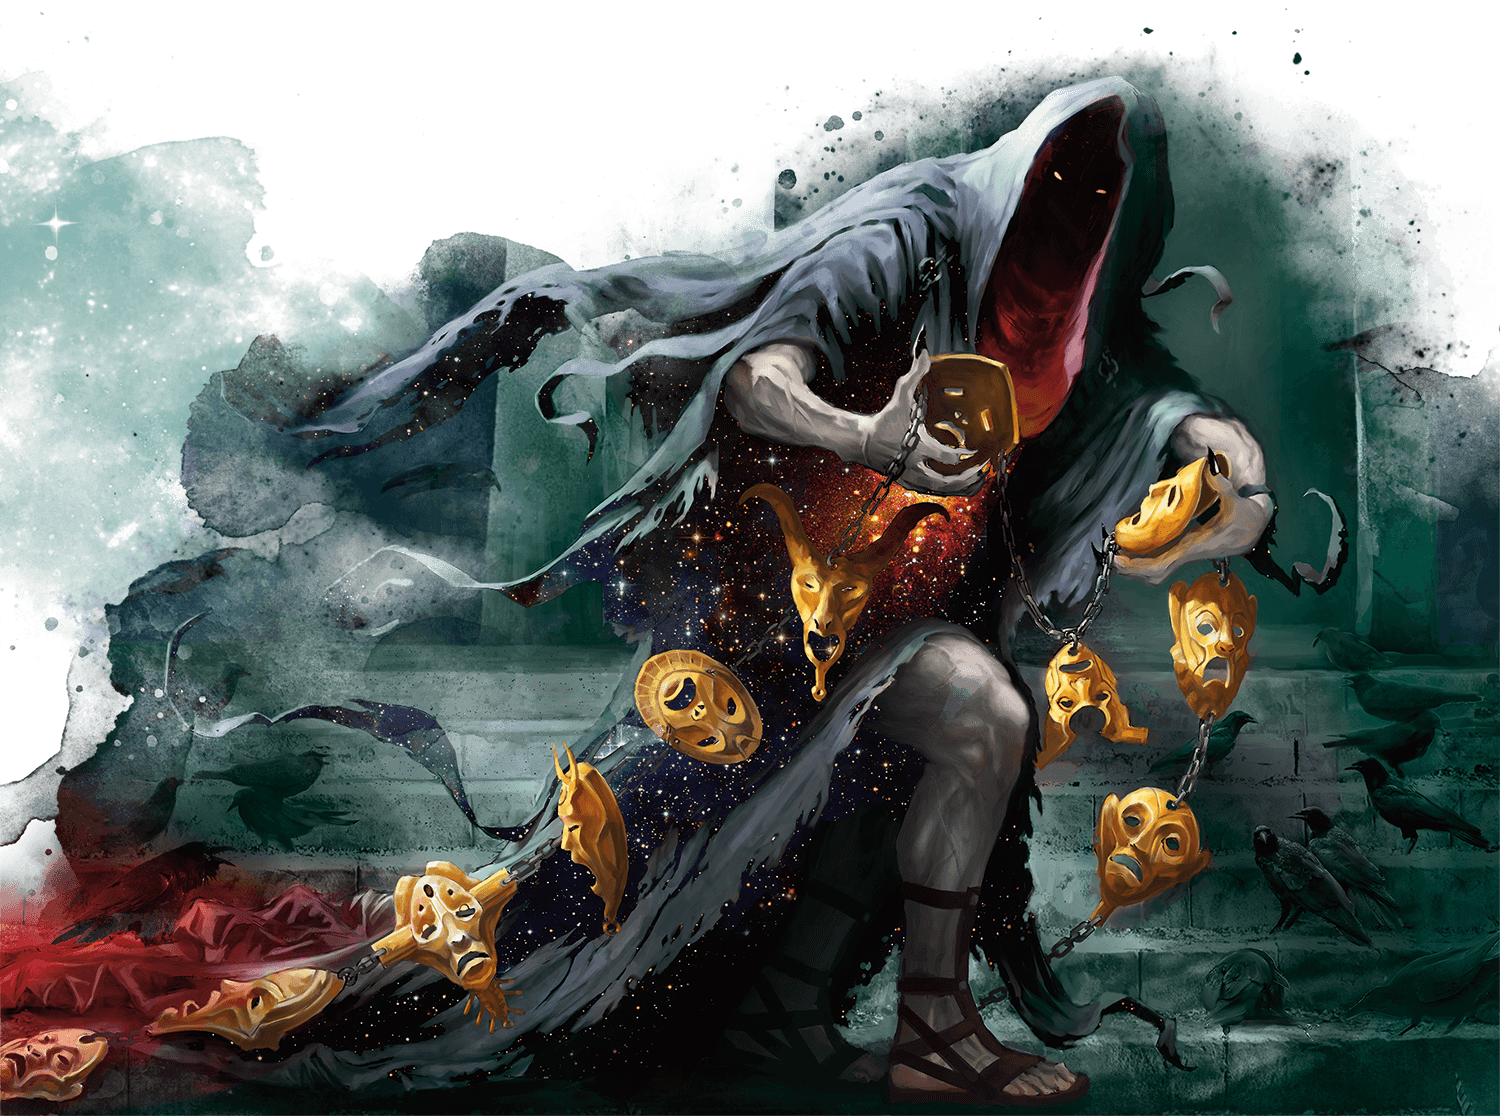
\includegraphics[width=\pdfpagewidth]{07spellcasting/img/10erebos.png}};
    % \end{tikzpicture}

\newpage
% NOTE. I will probably end up filling this space with a corner image.

% !TEX root = ../main.tex
\section{Sympathy} \label{sec::sympathy}
% Red tide, fire, explode
% SCHOOLS: Queish, Eljur, !Flamespeaking

Born from the red tide, the sympathy doctrine focuses on tethering links, the exchange of properties, and the redirection of energy.
Oft called Sympathists, sympathy spellcasters establish sympathetic links of different kinds between objects and creatures, altering the world around them through these.

Sympathists manifest effects on the world via sympathetic links.
These links can be of three natures: heat, electric, and similarity.

\subparagraph{Heat Link}
    (see page \pageref{medium::ember}).
    Sympathy spellcasters can quickly produce great surges of energy around them, but these are useless without a spark to ignite them.
    Heat links are floating embers which act as these sparks.

\subparagraph{Electric Link}
    (see page \pageref{medium::charge}).
    In contrast with fire, sympathists don't require a spark to manifest energy in its most pure form: electricity.
    Nonetheless, without a charge to guide lightning, it just takes the shortest route towards the ground.
    Sympathists use electric links to apply these charges to creatures and objects around them, enabling them to direct lightning at foes and allies alike.

\subparagraph{Similarity Link}
    (see page \pageref{medium::tether}).
    Unlike other sympathetic mediums, similarity links connect creatures and objects to exchange properties between them.
    A sympathist can tether these links to, for example, increase the weight of a creature, change its form, levitate it, etc.

\subsection*{Flamespeaking} \label{ssec::flamespeaking}
    \textit{I see your future, mantled in ash.}

    The seers of Viphoger are said to be blessed by the gods, granted special sight that sees past our world, into the stars of Nyx and beyond.
    Even novice seers are able to glimpse the weave of fate, seeing the connections of destiny that bind us all.
    With proper training, years of practice, and a bit of intuition, the best soothsayers can foretell every possible future, not just those most likely.

    Flamespeakers are special seers, blessed by Purphoros, god of the forge.
    Through the god's divine power, they are able to see portents in the curl of smoke, the flicker of flames, and the patterns of ash.

    When you choose this spellcasting school, you learn the \textbf{Firetrap} heat link (see page \pageref{medium::firetrap}), as well as the \textbf{Screaming Bead} spell (see page \pageref{spell::screamingbead}).
    Neither the medium nor the spell count towards your known mediums and spells.

\pagebreak

    % \subsubsection{Flickering Future}
    %     With the exception of those blessed by Keranos, god of insight, or Klothys, god of destiny, the powers of a seer depend very little on which god they've received their sight from.
    %     The only variation is often in what they are able to see from their future --- for example, seers blessed by Erebos are usually haunted by visions of death, while those blessed by Nylea might know exactly when and where to find the quarry of their hunt.
    %
    %     Most seers receive their portents by sight, in moments when their eyes look beyond, to the weave of fate, and follow the tangled lines therein.
    %     The flamespeakers of Purphoros are different in that they are unable to see the weave directly, but instead view it in every spark and ember of fire.
    %     For them, fire and destiny are inextricable, one and the same, with the weave of destiny imprinted onto a fundamental force of the world.
    %
    % \subsubsection{Twist the Lines}
    %     While the method with which they view the future is novel, what truly sets the flamespeakers apart is their ability to twist and tangle the pieces of the weave that they can see.
    %     Like many of Purphoros' priests, the flamespeakers are vessels for the god's power, granting them control over fire in its many forms.
    %     But for the flamespeakers, control of fire means a control of destiny.
    %
    %     The flamespeakers are able to change the future as they see in the ashes.
    %     It requires great effort on their part, and the changes are rarely more than minor, but it can be done all the same.
    %     For this reason, the flamespeakers are highly sought after, especially by those who have been informed of a terrible fate destined to befall themselves or a loved one.

% !TEX root = ../main.tex
\section{Sigaldry} \label{sec::sigaldry}
\textbf{TODO}.
\newpage

% !TEX root = ../main.tex
\section{Alchemy} \label{sec::alchemy}
\textbf{TODO}.
\newpage

% Zuan can be moved up to 4 meters as a free action.

% !TEX root = ../main.tex
\section{Thaumaturgy} \label{sec::thaumaturgy}
\textbf{TODO}.
\newpage

% !TEX root = ../main.tex
\section{Spellcasting Feats}
All feats in this section require the \textbf{Spellcaster} feat (see page \pageref{feat::spellcaster}), except naturally for the feat itself.

% === MAGIC SCHOOLS ============================================================ %
% All schools of magic require at least one rank in SPELLCASTING and one rank in a skill or tool (depends on the school).
% Spellcasting
% Bonereading (bonecarving tools)
% Wordbinding (two ranks in standard language - second is basic true speech)
% Windherding (acrobatics)
% Sigaldry (two ranks in naenk tongue - first to learn language, second to learn shinerunes)
% Psionics (two ranks in mind speech - first is listening to zaloths that don't necessarily want to be heard, second is feelspeech, and third is actual mind speech)
% Thaumaturgy (science)
% Tidal Manipulation (religion)
% Fleshshaping (nature)

\begin{DndTable}[width=\linewidth, header=General Spellcasting Feat List]{ll}
    \textbf{Spellcasting Ability} & \textbf{Feat}                                                                \\
    \textbf{---}                  & \textbf{Spellcaster}            (page \pageref{feat::spellcaster})           \\
    \textbf{---}                  & \textbf{Avid Caster}            (page \pageref{feat::avidcaster})            \\
    Intelligence                  & \textbf{Careful Spell}          (page \pageref{feat::carefulspell})          \\
    Intelligence                  & \textbf{Heedful Aim}            (page \pageref{feat::heedfulaim})            \\
    Intelligence                  & \textbf{Seeking Spell}          (page \pageref{feat::seekingspell})          \\
    Intelligence                  & \textbf{Spell Sniper}           (page \pageref{feat::spellsniper})           \\
    Intelligence                  & \textbf{Tactical Wit}           (page \pageref{feat::tacticalwit})           \\
    Wisdom                        & \textbf{Durable Magic}          (page \pageref{feat::durablemagic})          \\
    Wisdom                        & \textbf{Extended Spell}         (page \pageref{feat::extendedspell})         \\
    Wisdom                        & \textbf{Focused Casting}        (page \pageref{feat::focusedcasting})        \\
    Wisdom                        & \textbf{Numerous Mediums}       (page \pageref{feat::numerousmediums})       \\
    Wisdom                        & \textbf{Twinned Spell}          (page \pageref{feat::twinnedspell})          \\
    Charisma                      & \textbf{Empowered Spell}        (page \pageref{feat::empoweredspell})        \\
    Charisma                      & \textbf{Heightened Spell}       (page \pageref{feat::heightenedspell})       \\
    Charisma                      & \textbf{Quick Casting}          (page \pageref{feat::quickcasting})          \\
    Charisma                      & \textbf{Spontaneous Deflection} (page \pageref{feat::spontaneousdeflection}) \\
    Charisma                      & \textbf{Subtle Spell}           (page \pageref{feat::subtlespell})
\end{DndTable}

\begin{DndTable}[width=\linewidth, header=School Spellcasting Feat List]{ll}
    \textbf{Doctrine or School} & \textbf{Feat}                                                                \\
    Sympathy 1                  & \textbf{Comforting Flame}       (page \pageref{feat::comfortingflame})       \\
    Sympathy 1                  & \textbf{Emboldening Connection} (page \pageref{feat::emboldeningconnection}) \\
    Sympathy 1                  & \textbf{Forced Disattachment}   (page \pageref{feat::forceddisattachment})   \\
    Sympathy 1                  & \textbf{Scalding Ember}         (page \pageref{feat::scaldingember})         \\
    Sympathy 1                  & \textbf{Tamed Lightning}        (page \pageref{feat::tamedlightning})        \\
    Sympathy 1                  & \textbf{Violent Discharge}      (page \pageref{feat::violentdischarge})      \\
    Sympathy 2                  & \textbf{Overexertion}           (page \pageref{feat::overexertion})          \\
    Sympathy 2                  & \textbf{Stored Energy}          (page \pageref{feat::storedenergy})          \\
    Sympathy 2                  & \textbf{Storm Arteries}         (page \pageref{feat::stormarteries})         \\
    Sympathy 2                  & \textbf{Sympathist's Fuel}      (page \pageref{feat::sympathistsfuel})       \\
    Flamespeaking               & \textbf{Guiding Spark}          (page \pageref{feat::guidingspark})          \\
    Flamespeaking               & \textbf{Message in the Ash}     (page \pageref{feat::messageintheash})       \\
    Flamespeaking               & \textbf{Prophetic Smoke}        (page \pageref{feat::propheticsmoke})        \\
    Flamespeaking               & \textbf{Stored Fuel}            (page \pageref{feat::storedfuel})            \\
    Flamespeaking               & \textbf{Twist the Lines}        (page \pageref{feat::twistthelines})         \\
    Flamespeaking               & \textbf{Vigorous Scream}        (page \pageref{feat::vigorousscream})
\end{DndTable}

\subsubsection{Avid Caster (2 FP)} \label{feat::avidcaster}
    You increase your spellcasting ability bonus by 2.
    You can take this feat two times.
\subsubsection{Careful Spell} \label{feat::carefulspell}
    When you cast a spell that forces other creatures to make a saving throw, you can protect one of those creatures from the spell's full force.

    You can take this feat two additional times.
    The first, you increase the number of creatures you can protect to 3.
    The second, the number of creatures you can protect is equal to your Intelligence modifier (minimum of 3).
    \paragraph{Requirements} Ability Modifier: Intelligence.
\subsubsection{Comforting Flame} \label{feat::comfortingflame}
    All allied creatures within 3 meters of at least one ember gain a +1 bonus to their AC.
    \paragraph{Requirements} Doctrine: Sympathy.
\subsubsection{Durable Magic} \label{feat::durablemagic}
    When you cast a spell that requires concentration, you can spend an additional action to still yourself while casting.
    While you maintain concentration on the spell, you have a +2 bonus to AC and all saving throws.
    \paragraph{Requirements} Ability Modifier: Wisdom.
\subsubsection{Emboldening Connection} \label{feat::emboldeningconnection}
    All creatures connected via a similarity link gain a +1 bonus to all saving throws for each other creature attached through the link.
    \paragraph{Requirements} Doctrine: Sympathy.
\subsubsection{Empowered Spell (2FP)} \label{feat::empoweredspell}
    When you roll damage for a spell, you can spend a spell point to reroll a number of the damage dice up to your Charisma modifier (minimum of one).
    You must use the new rolls.
    \paragraph{Requirements} Ability Modifier: Charisma.
\subsubsection{Extended Spell} \label{feat::extendedspell}
    When you cast a spell that has a duration of 1 minute or longer, you can spend a spell point to double its duration, to a maximum of 24 hours.
    \paragraph{Requirements} Ability Modifier: Wisdom.
\subsubsection{Focused Casting (2FP)} \label{feat::focusedcasting}
    You gain a bonus to any Constitution saving throws you make to maintain concentration on a spell.
    The bonus equals your Wisdom modifier (minimum of +1).
    \paragraph{Requirements} Ability Modifier: Wisdom.
\subsubsection{Forced Disattachment} \label{feat::forceddisattachment}
    Whenever a sympathetic link is broken, all linked creatures are affected by a wave of lethargy.
    Until the end of your next turn, they can only take 2 actions per turn, their movement speed is reduced by 2 meters, and their AC is reduced by 2.
    \paragraph{Requirements} Doctrine: Sympathy.
\subsubsection{Guiding Spark} \label{feat::guidingspark}
    When you cast a spell that deals fire damage, you can expend one spell point to look into the trail of sparks and predict the creature's movements.
    Any ally that attacks the creature before the start of your next turn can roll a d4 and add the number rolled to the attack roll.
    \paragraph{Requirements} School: Flamespeaking, Competent proficiency with Glassblower's Tools.
\subsubsection{Heedful Aim (2FP)} \label{feat::heedfulaim}
    Your ranged spell attacks ignore half cover and three-quarters cover.
    \paragraph{Requirements} Ability Modifier: Intelligence.
\subsubsection{Heightened Spell} \label{feat::heightenedspell}
    When you cast a spell that forces a creature to make a saving throw to resist its effects, you can spend 3 spell points to give one target of the spell disadvantage
    \paragraph{Requirements} Ability Modifier: Charisma.
\subsubsection{Message in the Ash (2 FP)} \label{feat::messageintheash}
    You can call on Purphoros to intervene on your behalf when your need is great.

    Describe the assistance you seek, and roll percentile dice.
    If you roll a number equal to or lower than your level, Purphoros intervenes.
    The DM chooses the nature of the intervention.
    If the deity intervenes, you can't use this feat again for a week.
    Otherwise, you can use it again after you finish a short rest.

    At 20th level, your call for intervention succeeds automatically, no roll required.
    \paragraph{Requirements} School: Flamespeaking, Expert proficiency with Glassblower's Tools.
\subsubsection{Numerous Mediums} \label{feat::numerousmediums}
    The maximum number of mediums of the same type you can maintain is increased by one.

    You can take this feat two additional times, increasing the maximum number of mediums by one each time.
    \paragraph{Requirements} Ability Modifier: Wisdom.
\subsubsection{Overexertion (2FP)} \label{feat::overexertion}
    As a free action, you can choose to gain a number of spell points equal to a third of your total spell points.
    When you do this, you gain one level of exhaustion, and gain vulnerability to cold damage until you take a short rest.
    \paragraph{Requirements} Doctrine: Sympathy, MCA: Upgraded Spellcasting.
\subsubsection{Prophetic Smoke} \label{feat::propheticsmoke}
    When you deal fire damage to a creature, you can expend one spell point to look into the pattern of smoke and foresee the creature's movements.
    The next attack the creature does against you is made with disadvantage.
    \paragraph{Requirements} School: Flamespeaking, Competent proficiency with Glassblower's Tools.
\subsubsection{Quick Casting (2FP)} \label{feat::quickcasting}
    When you cast a spell that has a casting time of 2 or more actions, you can spend 3 spell points to reduce the casting time by 1 action for this casting.
    \paragraph{Requirements} Ability Modifier: Charisma.
\subsubsection{Scalding Ember} \label{feat::scaldingember}
    Upon starting its turn within a meter of at least one ember, a creature takes 1d6 fire damage.
    \paragraph{Requirements} Doctrine: Sympathy.
\subsubsection{Seeking Spell} \label{feat::seekingspell}
    If you make an attack roll for a spell and miss, you can spend 2 spell points to reroll the d20, and you must use the new roll.
    \paragraph{Requirements} Ability Modifier: Intelligence.
\subsubsection{Spell Sniper (2FP)} \label{feat::spellsniper}
    When you cast a spell hat has a range of 1 meter or greater, you can spend one spell point to double the range of the spell.

    When you cast a spell that has a range of touch, you can spend 1 spell point to make the range of the spell 6 meters.
    \paragraph{Requirements} Ability Modifier: Intelligence.
\subsubsection{Spellcaster (2 FP)} \label{feat::spellcaster}
    By joining one spellcasting school of your choice, you learn how to cast spells.
    Pick a spellcasting school from the Spellcasting chapter (page \pageref{ch::spellcasting}).
    The benefits associated to each school are denoted on their respective sections.
    For the rules of spellcasting, see page \pageref{sec::spellcastingrules}.
\subsubsection{Spontaneous Deflection} \label{feat::spontaneousdeflection}
    You can weave your magic to fortify yourself against harm.
    When you are hit by an attack or you fail a saving throw, you can consume one spell point and use your reaction to gain a +2 bonus to your AC against that attack or a +4 bonus to that saving throw.
    \paragraph{Requirements} Ability Modifier: Charisma.
\subsubsection{Stored Energy (2FP)} \label{feat::storedenergy}
    Whenever one of your embers fades, a creature is completely discharged, or a similarity link is broken, you feel a surge in energy.
    Once when you deal damage to a creature through any mean before the end of your next turn, it takes an additional 1d6 force damage.
    This damage increases by 1d6 when you reach 5th level (2d6), 11th level (3d6), and 17th level (4d6).
    \paragraph{Requirements} Doctrine: Sympathy, MCA: Upgraded Spellcasting.
\subsubsection{Stored Fuel} \label{feat::storedfuel}
    As part of a short rest, you can store a number of unspent spell points equal to your spellcasting ability modifier in a firetrap you are carrying.
    You can recover any number of these spell points at any point as a free action as long as you carry the firetrap.

    The maximum number of spell points that a firetrap can carry is equal to your spellcasting ability modifier.

    You can take this feat two additional times, multiplying the maximum number of points stored per short rest and the maximum number of spell points a firetrap can carry by two each time.
    \paragraph{Requirements} School: Flamespeaking, Skilled proficiency with Glassblower's Tools.
\subsubsection{Storm Arteries} \label{feat::stormarteries}
    Whenever you take fire or lightning damage, you gain one spell point.

    You can take this feat two additional times, increasing the number of spell points gained in this way by one for each time.
    \paragraph{Requirements} Doctrine: Sympathy, MCA: Upgraded Spellcasting.
\subsubsection{Subtle Spell} \label{feat::subtlespell}
    When you cast a spell, you can spend 1 additional spell point to cast it without any somatic or verbal components.
    \paragraph{Requirements} Ability Modifier: Charisma.
\subsubsection{Sympathist's Fuel} \label{feat::sympathistsfuel}
    When you make a Constitution saving throw to stave off the effects of extreme cold, you can choose to spend one spell point and automatically succeed.

    In addition, when you take cold damage, you can spend a number of spell points equal to half the number of damage dice of the attack (rounded down) to reduce the damage dealt by half.
    \paragraph{Requirements} Doctrine: Sympathy, MCA: Upgraded Spellcasting.
\subsubsection{Tactical Wit} \label{feat::tacticalwit}
    You gain a bonus to your initiative rolls equal to your Intelligence modifier.
    In addition, you can spend two spell points at the beginning of combat to roll initiative with advantage.
    \paragraph{Requirements} Ability Modifier: Intelligence.
\subsubsection{Tamed Lightning} \label{feat::tamedlightning}
    All creatures charged by you deal thunder damage equal to half the number of charges they have (rounded down) on all melee attacks.
    \paragraph{Requirements} Doctrine: Sympathy.
\subsubsection{Twinned Spell (2FP)} \label{feat::twinnedspell}
    When you cast a spell that targets only one creature and doesn't have a range of self, you can spend a number of spell points equal to half the total cost of the spell (rounded up) to target a second creature in range with the same spell (1 spell point if the spell has a cost of 0).

    To be eligible, a spell must be incapable of targeting more than one creature.
    \paragraph{Requirements} Ability Modifier: Wisdom.
\subsubsection{Twist the Lines (2FP)} \label{feat::twistthelines}
    As a reaction, you can expend two spell points to force a creature to reroll an attack roll.
    \paragraph{Requirements} School: Flamespeaking, Skilled proficiency with Glassblower's Tools.
\subsubsection{Vigorous Scream} \label{feat::vigorousscream}
    The radius of the \textbf{Screaming Bead} spell (see page \pageref{spell::screamingbead}) is extended to 6 meters.

    In addition, its range is extended to 12/18 mt.
    \paragraph{Requirements} School: Flamespeaking, Expert proficiency with Glassblower's Tools.
\subsubsection{Violent Discharge} \label{feat::violentdischarge}
    When a creature loses a charge via any means, it takes 1d6 thunder damage.
    \paragraph{Requirements} Doctrine: Sympathy.

% \newpage~
\newpage


% TODO: ! Thaumaturgy spellcasting school.
% TODO: ! Tortle alchemy-like chemistry, based on cooking to enhance effect of drugs and potions.
% TODO: ! Poison and alchemy stuff from followers of Pharika.
% TODO: ! Warchanting - using drugs and rituals to enhance rage in the name of Mogis.
    % Rage burns a spell point each turn while its activated, and other effects can use more spell points.
    % Rage has all the normal effects from the barbarian class.
    % lv 2: burn one additional spell point to gain one action during your turn.
    % lv 3: burn two spell points to ignore the multiple attack penalty while raging.

    % Bloodhorn Minotaurs
    % Named for their blood-caked horns, the Bloodhorn minotaurs have ragged claws to supplement their charges and gores. Gleeful in their brutality, they slaughter and devour any intruders they encounter in the badlands, and particularly value the bone marrow of young humans. They take pride in their overlarge, razor-sharp horns.

    % Felhide Minotaurs
    % The notoriously dour Felhide minotaurs are descended from the warlord Thyrogog of the Ashlands. The Theriad recounts the brute's defeat and the loss of his great axe, Goremaster. Viewing Thyrogog's defeat as a divine sign, the warlord's descendants retreated into the Ashlands.

    % Burial rites among the Felhide minotaurs involve devouring those who fell in battle, to remove their shame from memory and fuel the survivors' revenge. Should another scavenger reach a fallen Felhide before the rest of the band can eat the dead minotaur's remains, the minotaurs mobilize to track down as much of their dead comrade's body as possible.

    % Ragegore Minotaurs
    % Ragegore minotaurs are the most ferocious of their kind, deeply infected by the bloodlust of Mogis. Ragegores never withdraw from a battle, entering a frenzy of furious delight at the sight of an enemy's blood. While in the heat of battle, a Ragegore minotaur seems to feel no pain and barely notices wounds that would kill a human. Some Ragegores have been known to fall dead immediately at the cessation of battle, their life sustained only by their fury.
